\documentclass{article}
\usepackage{amsmath}
\usepackage{amsfonts}
\usepackage{tikz}
\usepackage{qtree}
\usetikzlibrary{automata,arrows}

\begin{document}

\section*{Student Information}
Name: Batuhan Akçan \\
ID: 2580181 \\

\section*{Answer 1}
\subsection*{1}
$ \equiv_0 : \{q_0, q_1, q_3, q_4\}, \{q_2, q_5\}$\\
$ \equiv_1 : \{q_0, q_1, q_3, q_4\}, \{q_2, q_5\} $\\
Since $\equiv_0 \; $is equal to$ \; \equiv_1$, the algorithm terminates. The equivalent minimal DFA is:\\

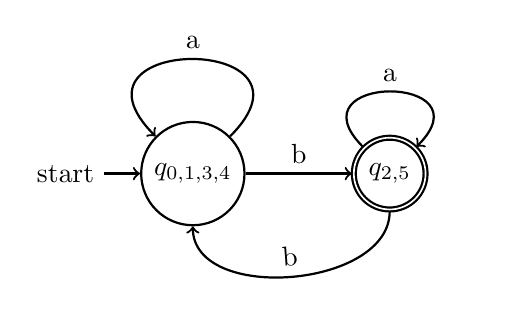
\begin{tikzpicture}[node distance={25mm}, thick, main/.style = {draw, circle}] 

\node[initial, state] (1) {$q_{ 0,1,3,4}$};
\node[state, accepting] (2) [right of=1] {$q_{ 2,5}$}; 

\draw[->] (1) to [out=45,in=135,looseness=5] node[midway, above, sloped, pos=0.5] {a} (1);
\draw[->] (1) -- node[midway, above, sloped, pos=0.5] {b} (2);
\draw[->] (2) to [out=135,in=45,looseness=5] node[midway, above, sloped, pos=0.5] {a} (2);
\draw[->] (2) to [out=270,in=270,looseness=1] node[midway, above, sloped, pos=0.5] {b} (1);

\end{tikzpicture}

\subsection*{2}
$[q_{0,1,3,4}] = a^* \cup (a^*ba^*b)^*$\\
$[q_{2,5}] = a^*ba^*(ba^*ba^*)^* $

\subsection*{3}
Consider $a^i$ and $a^j$ where $i \neq j$. Let $i = k+2u-m.$ Then\\
$a^i \not\approx_{L'} a^j$ because $a^ib^mc^kd^u \in L$ and $a^jb^mc^kd^u \not\in L.$ There are infinitely many $i,j$ pairs because $m,k,u \in \mathbb{N}$, which means there are infinitely many $m,k,u.$ Thus, there are infinitely many equivalence classes. Hence, by MyHill-Nerode Theorem, $L'$ is not regular.

\section*{Answer 2}
\subsection*{1}
$G = (V,\Sigma, R, S)$ where\\
$V = \{S, a, b\}$\\
$\Sigma = \{a,b\}$\\
$R = \{S\rightarrow b,\; S\rightarrow bS,\; S\rightarrow Sb,\; S\rightarrow bSa,\; S\rightarrow aSb\}$
\subsection*{2}
$G = (V,\Sigma, R, S)$ where\\
$V = \{S, 0, 1, 2\}$\\
$\Sigma = \{0,1,2\}$\\
$R = \{S\rightarrow e,\; S\rightarrow 0S1,\; S\rightarrow 1S0,\; S\rightarrow 1S2,\; S\rightarrow 2S1\}$
\subsection*{3}
$G = (V,\Sigma, R, S)$ where\\
$V = \{S, 0, 1\}$\\
$\Sigma = \{0,1\}$\\
$R = \{S\rightarrow 0,\; S\rightarrow 1,\; S\rightarrow 1S0,\; S\rightarrow 0S1,\; S\rightarrow 0S0,\; S\rightarrow 1S1\}$\\

\Tree[ .S 0 [ .S 0 [.S 1 [.S 1 ] 1 ] 0 ] 0 ]

\section*{Answer 3}
\subsection*{1}
$L_1 = \{ w \in \{0,1\}^* \; | \; w = 0(0\cup 1)^*0\; \cup \; 1(0\cup 1)^*1 \; \cup \; e \}$

\subsection*{2}
$L_2 = \{w \in \{0,1\}^* \; | \; w = (0\cup 1)^*1(0\cup 1)^*1(0\cup 1)^*\}$







\end{document}